\documentclass[aps,prb,showpacs,amsmath,amssymb,superscriptaddress]{revtex4-2}

\usepackage{tabularx}
\usepackage{bm}
%\usepackage[demo]{graphicx}
\usepackage{graphicx}

\usepackage{hyperref}
\hypersetup{colorlinks=true,urlcolor= blue,citecolor=blue,linkcolor= blue,bookmarks=true,bookmarksopen=false}

\usepackage{color}

\usepackage{amsmath,mathtools}
\usepackage{multirow}
\usepackage{dcolumn}
\usepackage{amssymb,amscd,xypic,bm,wasysym}
\usepackage{float}
\usepackage{cleveref}
\usepackage[caption=false,position=top,captionskip=0pt,farskip=0pt]{subfig}
\captionsetup[subfigure]{justification=raggedright,singlelinecheck=false}


\newcommand{\Red}[1]{\textcolor{red}{#1}}
%\newcommand{\vb}[1]{\boldsymbol{#1}}
\usepackage{soul}

% reset vec and hat style to a bold type
\let\oldhat\hat
\renewcommand{\hat}[1]{\oldhat{\mathbf{#1}}}
\renewcommand{\vec}[1]{\mathbf{#1}}
% stretches the vertical spacing of arrays/matrices
\renewcommand{\arraystretch}{1.5}
\setlength{\jot}{10pt}

\newcommand{\ham}{\mathcal{H}}
\newcommand{\cc}{c^{\dagger}}
\newcommand{\de}{\Delta}


\begin{document}

\title{Supplementary Material for ``Superconducting triangular islands as a platform for manipulating Majorana fermions"}

\author{Aidan Winblad}
\affiliation{Department of Physics, Colorado State University, Fort Collins, CO 80523, USA}

\author{Hua Chen}
\affiliation{Department of Physics, Colorado State University, Fort Collins, CO 80523, USA}
\affiliation{School of Advanced Materials Discovery, Colorado State University, Fort Collins, CO 80523, USA}

\maketitle

\section{Many-body Berry phase calculation for the 3-site Kitaev triangle}

A many-body Berry phase calculation was calculated for the 3-site Kitaev triangle using Python3 and Mathematica.
To start we use the Hamiltonian presented in the paper,

\begin{equation}\label{eq:HBdG}
  \ham = \sum_{\langle j l \rangle} (-te^{i\phi_{jl}}\cc_{j} c_l + \de e^{i\theta_{jl}} c_{j} c_l + {\rm h.c.}) - \sum_{j} \mu \cc_j c_j,
\end{equation}
We write the creation and annihilation operators in Fock space for three fermions with the following basis

\begin{align*}
  \{&|0,0,0 \rangle, \\
  &|1,0,0 \rangle, |0,1,0 \rangle, |0,0,1 \rangle, \\
  &|0,1,1 \rangle, |1,0,1 \rangle, |1,1,0 \rangle, \\
  &|1,1,1 \rangle\} = \{|0\rangle, |1\rangle, \dots, |7\rangle\}.
\end{align*}
The creation(annihilation) operators in this space are defined as

\begin{align}
  \cc_j |n_1,\dots,n_j, \dots\rangle = (n_j+1)^{1/2}(-1)^{s_j}|n_1,\dots,n_j+1,\dots\rangle, \\
  c_j |n_1,\dots,n_j, \dots\rangle = (n_j-1)^{1/2}(-1)^{s_j}|n_1,\dots,n_j-1,\dots\rangle,
\end{align}
where

\begin{equation}
  s_j =
  \begin{cases}
    \sum_{l=1}^{j-1} n_l & \text{if $j>1$} \\
    0 & \text{if $j = 1$}
  \end{cases}
  .
\end{equation}

We make use of the Majorana fermion (MF) basis using $\cc_j = \dfrac{1}{2} (a_j - i b_j)$.
In this minimal model we will assume the fermionic ground state represents the bottom two vertices of the triangle hosting MFs which appears as

\begin{equation}
  f = \dfrac{1}{2} ( a_1 + i b_2 )
\end{equation}
and the fermionic number operator is simply $f^{\dagger} f$.

Next, we solve for the ground state eigenvalues and eigenvectors of the Hamiltonian in the initial configuration, $\bm \phi_1$, $(\ham-\epsilon_j)|\psi_j\rangle_0=0$.
The Unitary ground state operator is made from the two degenerate ground state column eigenvectors

\begin{equation}
  U_{gs} = [\psi_0,\  \psi_1]
  \end{equation}
Similarly, we find the Unitary number operator, $U_n$, from the fermionic ground state solving the following eigenvalue problem $f^{\dagger}f|\eta\rangle = \lambda|\eta\rangle$.
We can now project the Unitary ground state to fermionic ground state basis with

\begin{equation}
  \tilde{U}_i = U_{gs} U_{n} = [ |0\rangle_i,\  |1\rangle_i],
\end{equation}
in other words, this represents the initial two ground state MFs.

To carry out the Berry phase calculation we next need to adiabatically ``rotate'' the vector potential field by following the linearly interpolated closed parameter path described in the main text.
For each small increment $\delta$ of the Hamiltonian for a varying $\bm \phi$ we can create a projection operator from their degenerate ground states, $P_{\delta} = \sum_j^{0,1} \leftindex_{\delta}|\psi_j\rangle \langle \psi_j |_{\delta}$.
The ground state manifold can be well approximated with small $\delta$ by

\begin{equation}
  M_{jl} = \tilde{U}_f^{\dagger}\  P_{f-\delta} \dots P_{i+\delta}\  \tilde{U}_i.
\end{equation}
We found the global phase factor to be $e^{i\vartheta} \approx e^{i0.37\pi}$ and the ground states were out of phase by $0.499999995\pi \sim \dfrac{\pi}{2}$.

Using the same process we calculated the Berry phase for a rotating constant vector potential for a 3-site kitaev triangle.
Due to the precise parameter space of a Kitaev triangle the rotation creates hybridized ground state Majorana-like fermions and essentially bulk modes.
This causes their Fock space energies to differ enough they are no longer degenerate which I think causes the phases to accumalate at different rates leading to the undesired phase differences between the two ground states.


\section{Majorana corner modes for finite-width triangles}

\begin{figure}
  \hspace{28pt}
  \subfloat[]{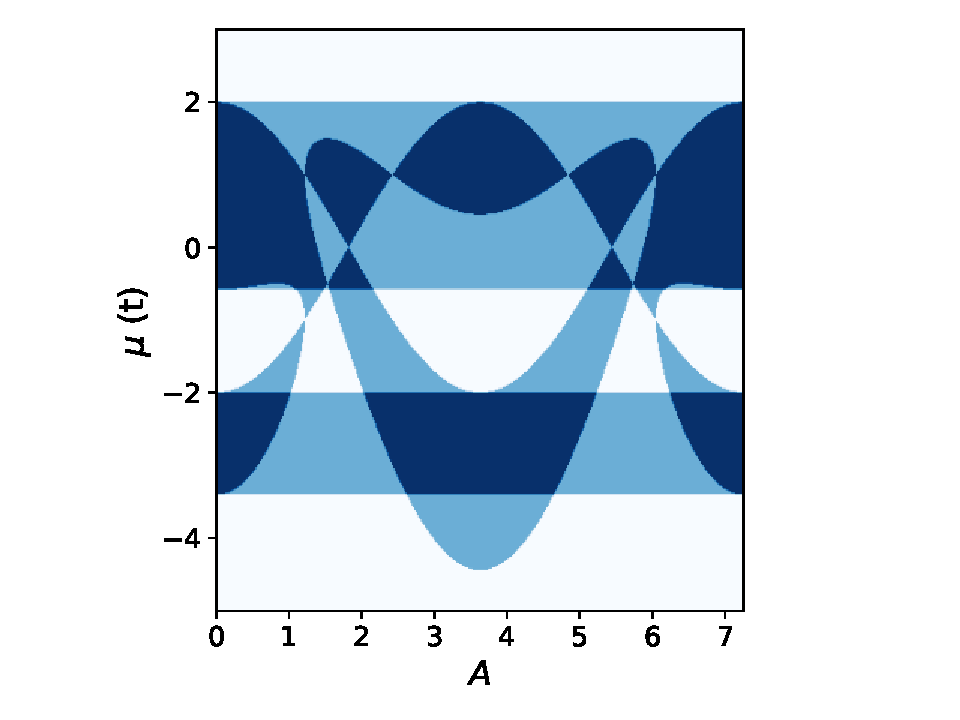
\includegraphics[width=0.65\textwidth]{./figures/supp/topological-phase-diagram-1pi6-n-3.pdf}} \\
  \vspace{-20pt}
  \subfloat[]{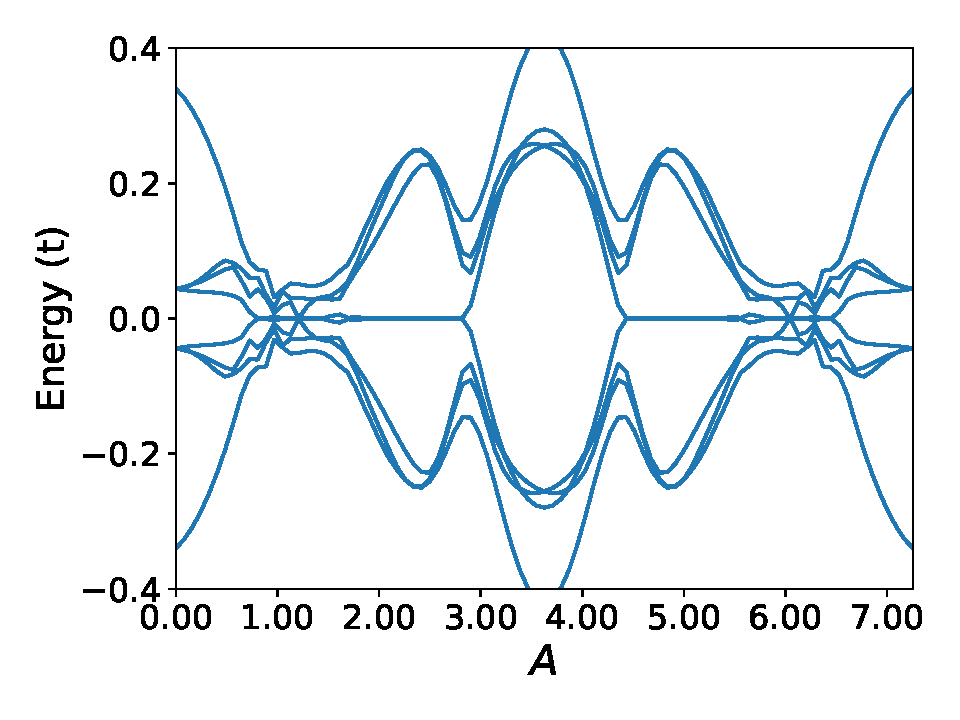
\includegraphics[width=0.46\textwidth]{./figures/supp/spectral-flow-nr-50-w-3-mu-1_6.pdf}} \\
  \hspace{70pt}
  \subfloat[]{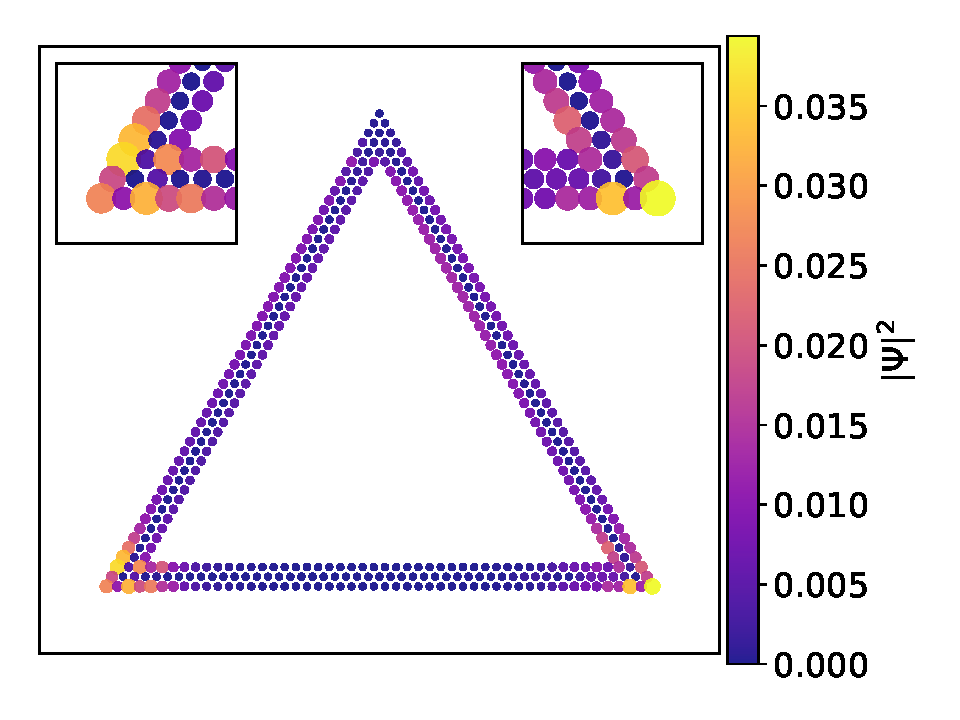
\includegraphics[width=0.50\textwidth]{./figures/supp/GS-A-2_74-nr-50-w-3-mu-1_6.pdf}}
  \caption{(a) Topological phase diagram for a $W=3$ hollow triangle obtained by overlapping the $\mathcal{M}(A, \mu)      $ plots of 1D chains with $\mathbf A = A\hat{y}$ and $\mathbf A = A(\frac{\sqrt{      3}}{2}\hat{x}+\frac{1}{2}\hat{y})$. Color scheme: white---$\mathcal{M}=1$, dark blue---$\mathcal{M}=-1$, light blue---$\mathcal{M}=0$ (b) Near-gap BdG eigen-energies vs $A$ for a finite triangle with edge length $L=50$, $W=3$, and $\mu=1.6$. (c) BdG eigenfunction $|\Psi|^2$ summed over the two zero modes at $A=2.4709$}
  \label{fig: supp pd}
\end{figure}

It may be more realistic to calculate a finite-width, or hollow, triangular islandswith a constant vector potential applied.
Figure \ref{fig: supp pd} shows the numerical results for a hollow triangle of length, $l=50$, and edge width, $w=3$.
For the Majorana number (MN) or topological phase (TP) diagram we assume each edge is a long enough ribbon we calculate the MN for the relative angle the vector potential makes with them.
Like in the triangular chain, main text, the vector potentials affect on MN is symmetric about the edges axis, i.e. we need only worry about $0 \leq \phi \leq \pi/2$.
We see agreement between the TP diagram and near-gap eigen-energies where MFs should lie.
The Eigenfunction for $A=2.7409$ shows that we do indeed get MFs at the bottom vertices of the hollow triangle island.

\begin{figure}
  \subfloat[]{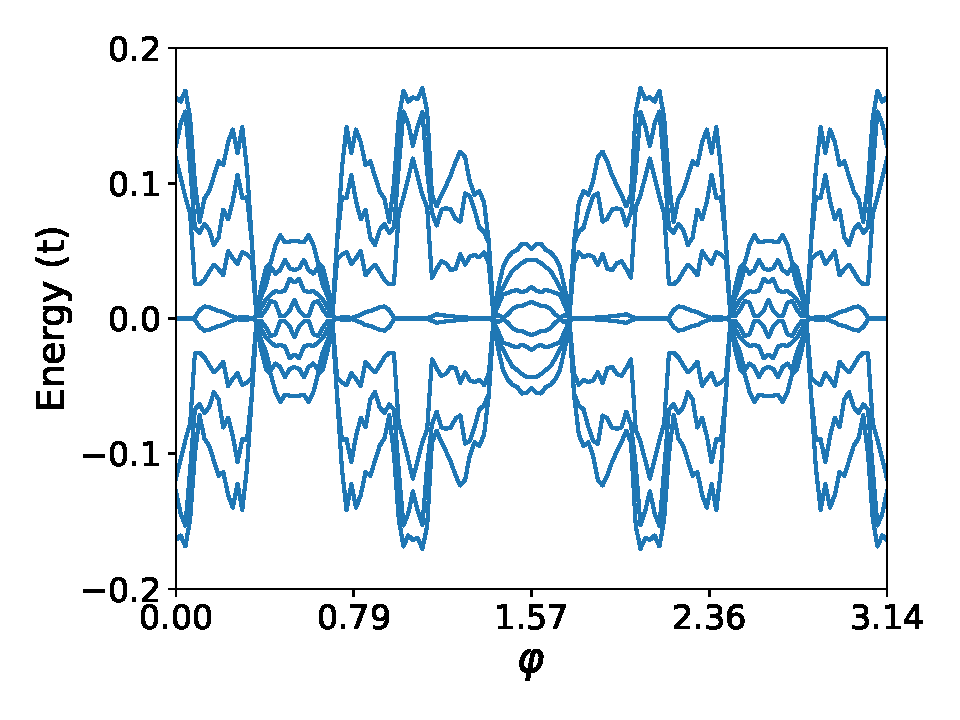
\includegraphics[width=0.4\textwidth]{./figures/supp/spectral-flow-w-3.pdf}}
  \subfloat[]{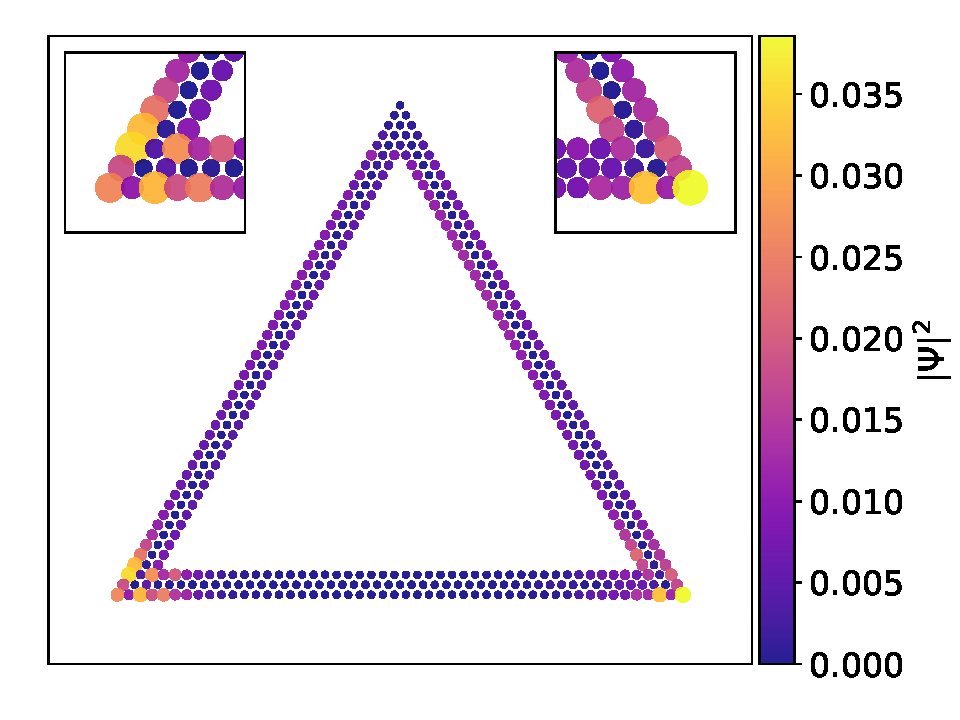
\includegraphics[width=0.4\textwidth]{./figures/supp/GS-T-Square-w-3.pdf}} \\
  \subfloat[]{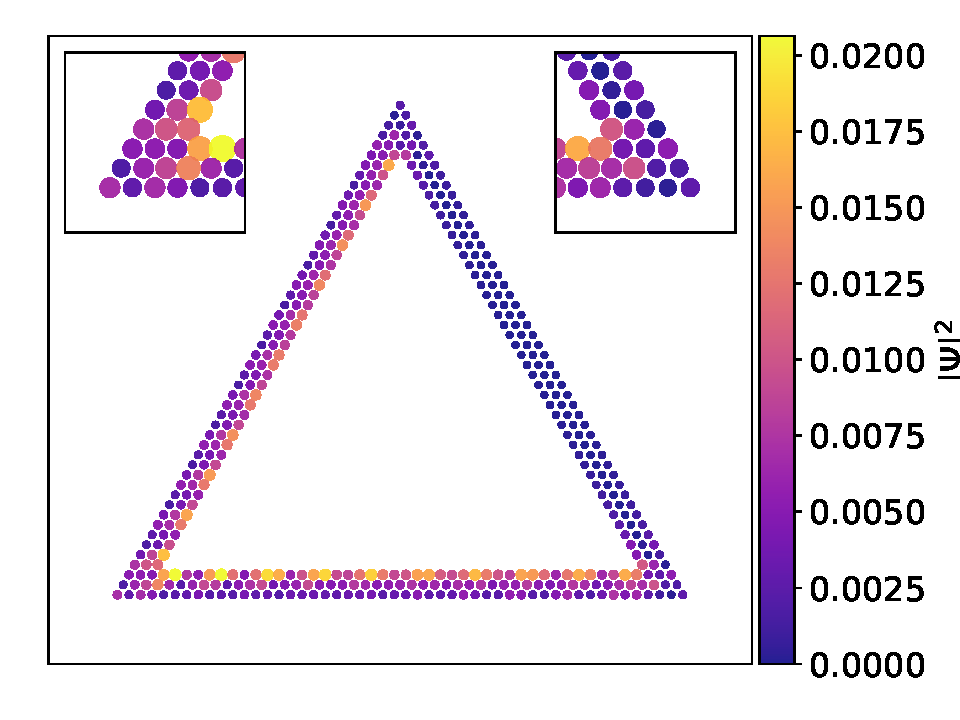
\includegraphics[width=0.4\textwidth]{./figures/supp/GS-T-Circle-w-3.pdf}}
  \subfloat[]{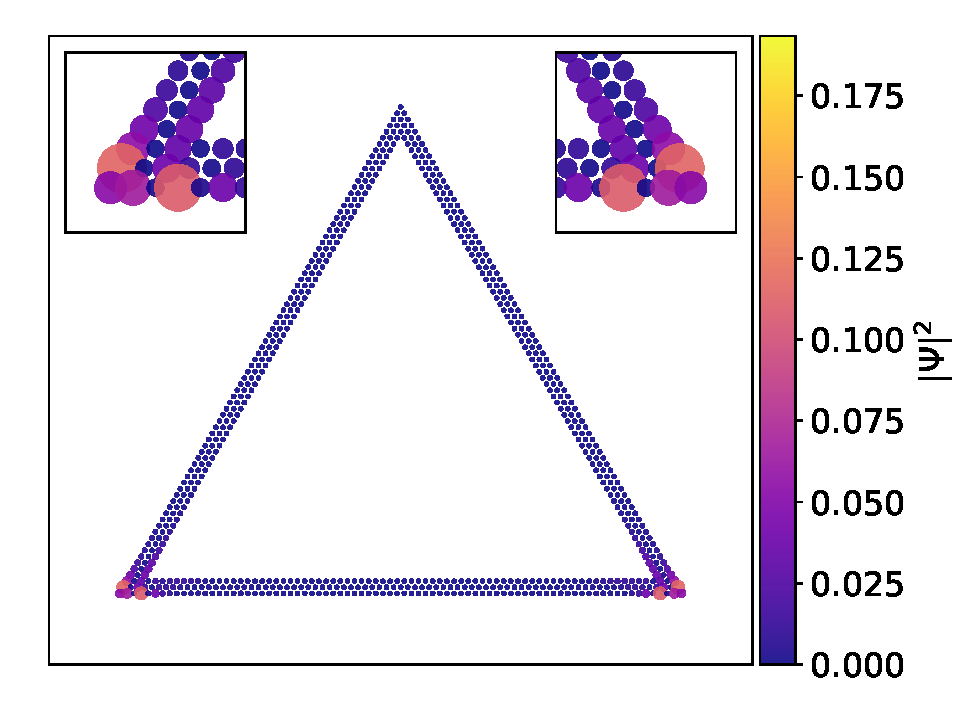
\includegraphics[width=0.4\textwidth]{./figures/supp/GS-T-Diamond-w-3.pdf}}
  \caption{(a) Spectral flow of a hollow triangle with $W=3$, $L=50$, $\mu=1.6$,       and $A=2.75$ with increasing rotation angle $\varphi$, defined through $\mathbf A = A(\cos\varphi \hat{x} + \sin\varphi \hat{y})$. (b-d) BdG eigenfunction $|\Psi|^2$ summed over the two zero modes at $\varphi = 0, \frac{\pi}{6}$, and $\frac{\pi}{3}$, respectively.}
  \label{fig: supp rotation}
\end{figure}

We now rotate the vector potential field to examine how the MFs move on a hollow triangle.
Figure \ref{fig: supp rotation} shows the spectral flow and eigenfunctions as we rotate $\varphi=0$ to $\varphi=\pi$.
It appears that MFs host at the corners of the edge that is perpendicular to the vector potential field and still also when the vector potential is parallel, albeit more of an edge state as seen in the spectral flow.
A longer length triangle helps drive the bulk/edge correspondence to force MFs at the corners of a hollow triangle.


\section{Braiding MZM in a small network of triangles}

It is now pertinent to see if we can use the previous results to interchange two MFs that are not paired together.
We initialize three triangular chains adjavent to each other, connecting their bottom corners together.
The left and right triangles initialize a constant vector potential with $\varphi=0$, while the middle island will initialize with $\varphi=\dfrac{\pi}{6}$.
Slowly rotating the middle triangle chains vector potential to $\varphi=\dfrac{\pi}{3}$ we see the the middle MFs swap which MF pair they are connected to.

\begin{figure}
  \subfloat[]{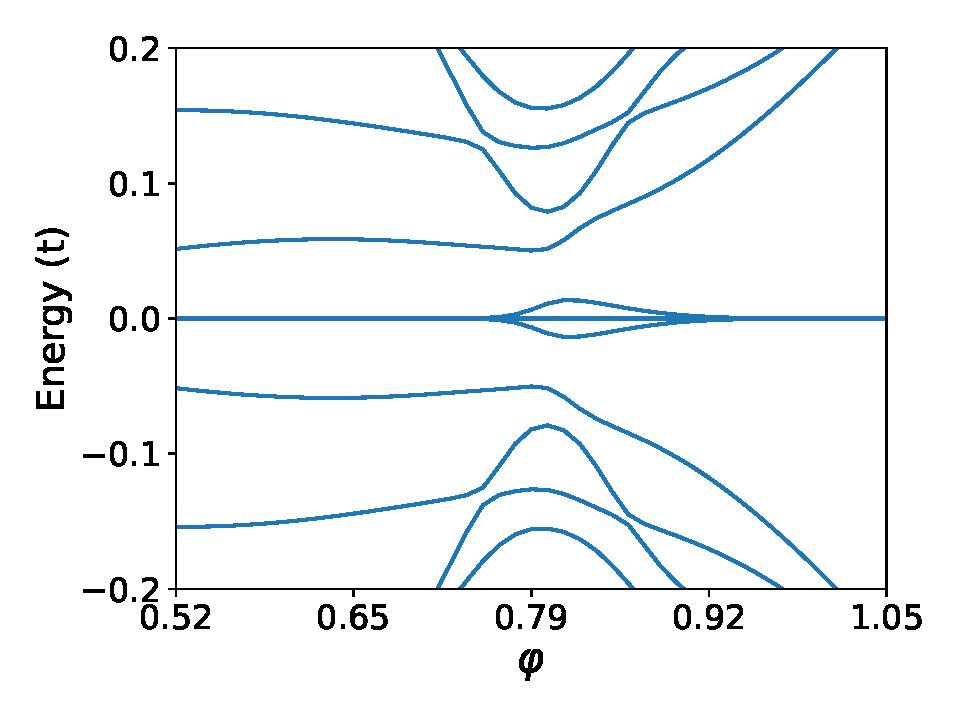
\includegraphics[width=0.4\textwidth]{./figures/supp/spectral-flow-braiding.pdf}} \\
  \subfloat[]{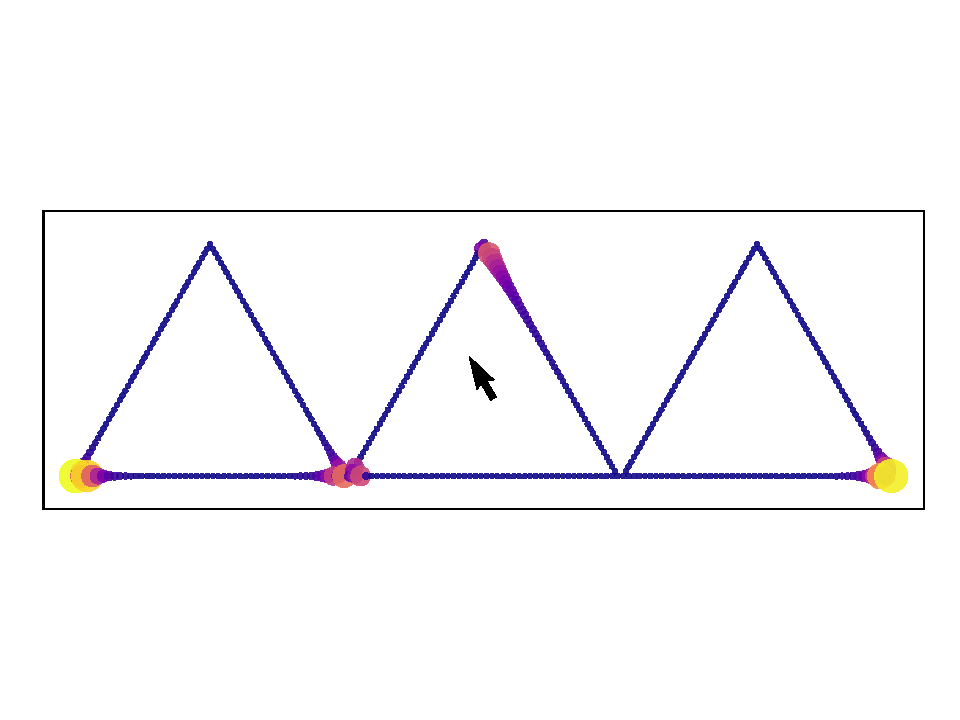
\includegraphics[width=0.4\textwidth]{./figures/supp/GS-Braid-0.pdf}}
  \subfloat[]{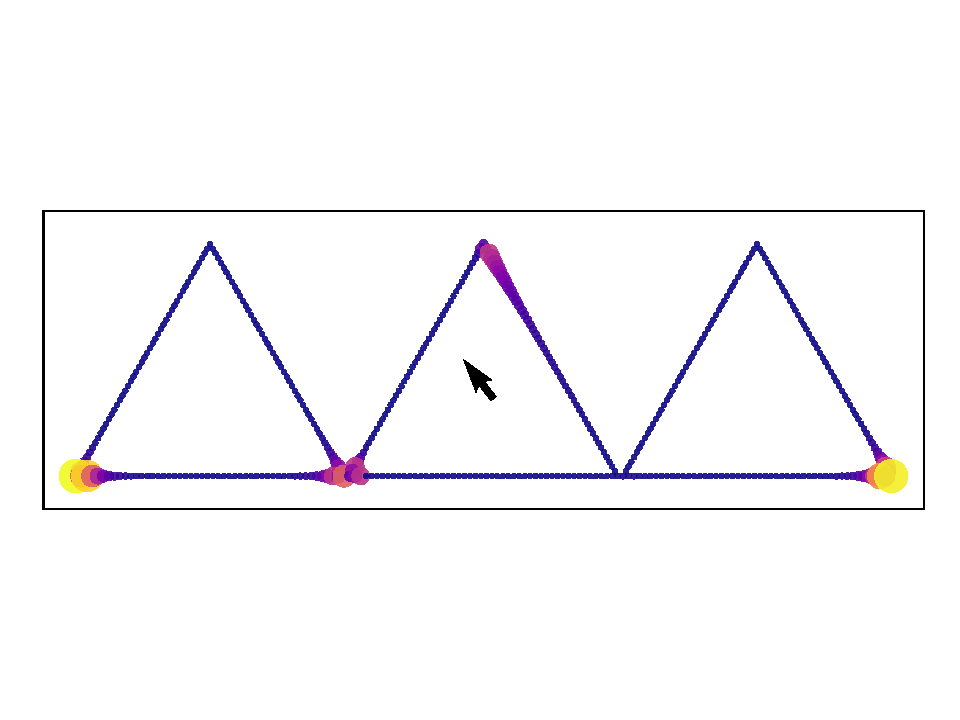
\includegraphics[width=0.4\textwidth]{./figures/supp/GS-Braid-1.pdf}} \\
  \vspace{-40pt}
  \subfloat[]{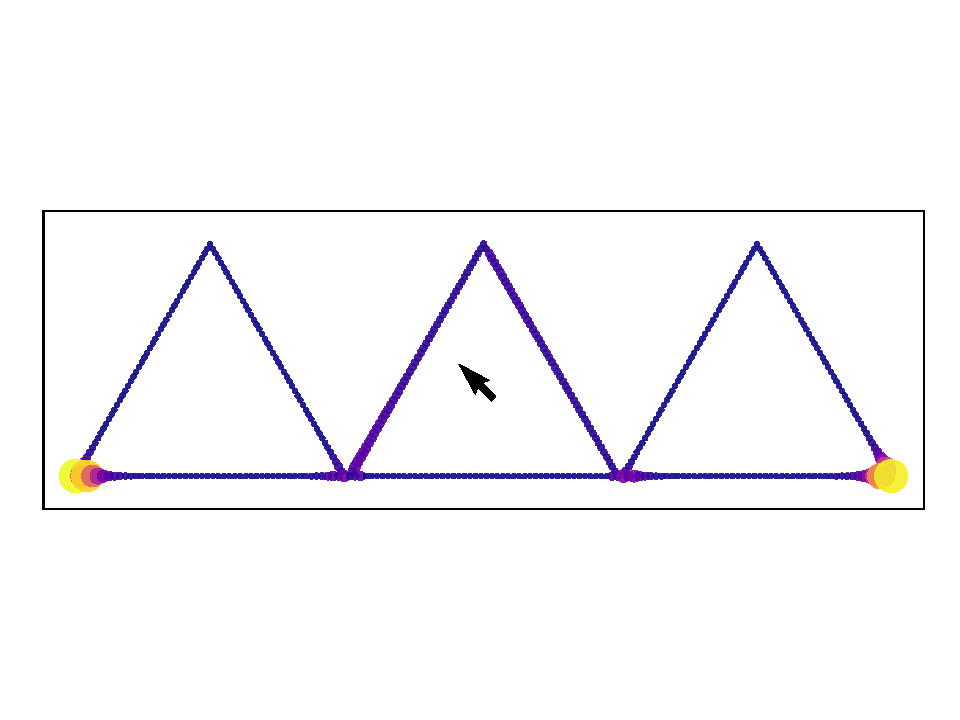
\includegraphics[width=0.4\textwidth]{./figures/supp/GS-Braid-2.pdf}}
  \subfloat[]{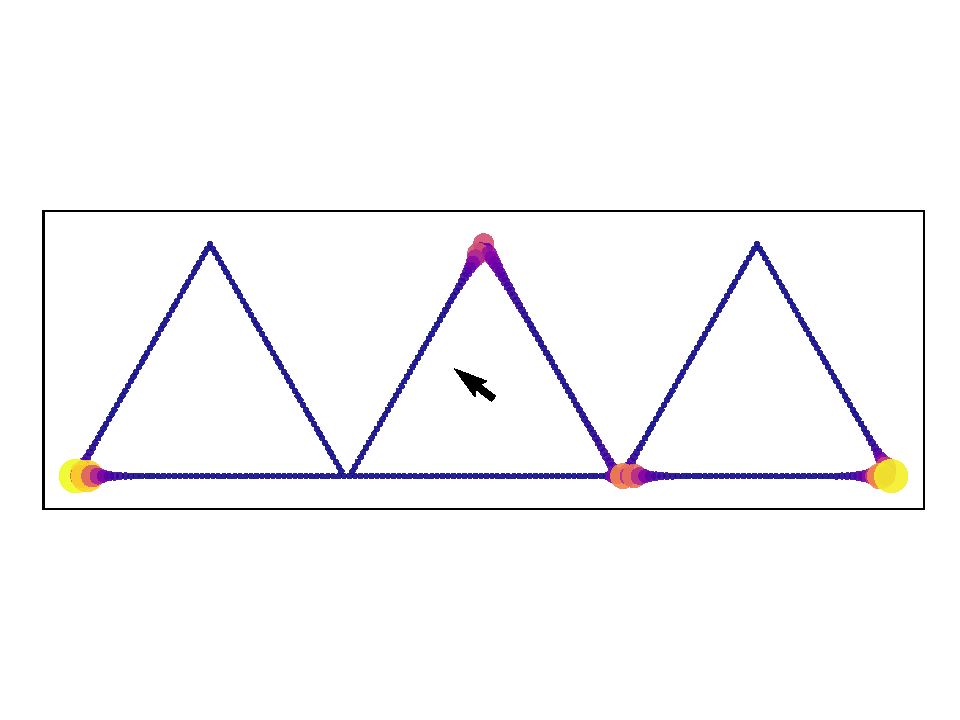
\includegraphics[width=0.4\textwidth]{./figures/supp/GS-Braid-3.pdf}} \\
  \vspace{-40pt}
  \subfloat[]{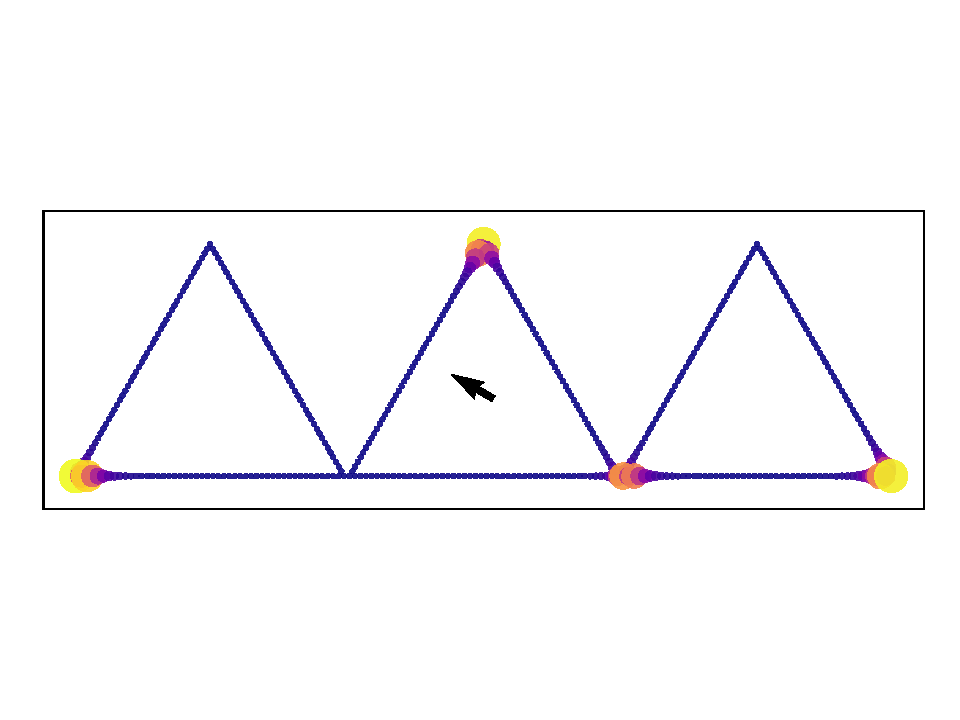
\includegraphics[width=0.4\textwidth]{./figures/supp/GS-Braid-4.pdf}}
  \caption{(a) Spectral flow of three triangular chains connected at their bottom certices in a row with $W=1$, $L=50$, and $\mu=1.6$. Each triangle has a vector potential field applied as $\mathbf A = A(\sin\varphi \hat{x} + \cos\varphi \hat{y})$, with $A=2.55$. The left and right trianlges have $\varphi=0$, while the middle triangle rotates $\varphi = \dfrac{\pi}{6}$ to $\varphi = \dfrac{\pi}{3}$. (b)-(f) BdG eigenfunction $|\Psi|^2$ summed over the four zero modes over the rotation of the middle triangles $\varphi$. }
\end{figure}

\bibliography{triag_ref}

\end{document}
